\documentclass[aps,prd,reprint,a4paper,nofootinbib,floatfix]{revtex4-2}
\usepackage[T1]{fontenc}
\usepackage[english]{babel}
\usepackage{mathptmx}
% English language rules and explicit embedding for the PSNFSS Times family.
% Standard TeX Live/MiKTeX distributions provide these URW Type 1 fonts.
% The overrides also work when a site's pdftex.map omits Base-14 outlines.
\ifdefined\pdfmapline
  \pdfmapfile{+rsfs.map}
  \pdfmapline{=ptmr8r NimbusRomNo9L-Regu "TeXBase1Encoding ReEncodeFont" <8r.enc <utmr8a.pfb}
  \pdfmapline{=ptmb8r NimbusRomNo9L-Medi "TeXBase1Encoding ReEncodeFont" <8r.enc <utmb8a.pfb}
  \pdfmapline{=ptmri8r NimbusRomNo9L-ReguItal "TeXBase1Encoding ReEncodeFont" <8r.enc <utmri8a.pfb}
  \pdfmapline{=ptmbi8r NimbusRomNo9L-MediItal "TeXBase1Encoding ReEncodeFont" <8r.enc <utmbi8a.pfb}
  \pdfmapline{=psyr StandardSymL <usyr.pfb}
  \pdfmapline{=rpsyr StandardSymL <usyr.pfb}
  \pdfmapline{=pzcmi8r URWChanceryL-MediItal "TeXBase1Encoding ReEncodeFont" <8r.enc <uzcmi8a.pfb}
  \pdfmapline{=pcrr8r NimbusMonL-Regu "TeXBase1Encoding ReEncodeFont" <8r.enc <ucrr8a.pfb}
\fi
\renewcommand{\ttdefault}{pcr}
\ifdefined\pdfgentounicode\pdfgentounicode=1\fi
\ifdefined\pdfinclusioncopyfonts\pdfinclusioncopyfonts=1\fi
\AtBeginDocument{\selectlanguage{english}\lefthyphenmin=2\righthyphenmin=3}
\emergencystretch=1em

\newcommand{\aiplotnote}{Plotting code was developed with ChatGPT/Codex assistance.}
\usepackage{amsmath,amssymb,amsthm}
\usepackage{booktabs,graphicx,url}
\usepackage[hidelinks]{hyperref}
\newtheorem{theorem}{Theorem}
\newtheorem{proposition}{Proposition}
\newtheorem{remark}{Remark}
\newcommand{\R}{\mathbb R}
\newcommand{\C}{\mathcal C}
\newcommand{\U}{\mathcal U}
\newcommand{\D}{\mathcal D}
\newcommand{\HH}{\mathcal H}
\newcommand{\norm}[1]{\left\|#1\right\|}
\newcommand{\dd}{\mathrm d}
\DeclareMathOperator*{\argmin}{\arg\,min}
\DeclareMathOperator*{\argmax}{\arg\,max}

\hypersetup{pdftitle={Slowly Rotating Perfect-Fluid Spheres with an Adiabatic Gas Surface},pdfauthor={Jan Olsina}}

\begin{document}
\title{Slowly Rotating Perfect-Fluid Spheres with an Adiabatic Gas Surface}
\author{Jan~Ol\v{s}ina}
\email{jan.olsina@gmail.com}
\thanks{ORCID: \href{https://orcid.org/0009-0003-9816-3958}{0009-0003-9816-3958}}
\affiliation{Independent Researcher, Prague, Czech Republic}
\date{17 October 2026}
\begin{abstract}
We construct a continuously stratified family of relativistic perfect-fluid spheres with exact background quadratures, algebraic frame dragging, and a finite surface satisfying $P\propto n^{5/3}$. A polynomial dragging profile determines the static geometry and gives the moment of inertia as a rational function of the family parameter. The Hartle--Thorne equations then supply the second-order rotational interior, matched to a vacuum exterior with an independently determined quadrupole. Published homogeneous-star and polytropic results benchmark the rotational calculation. Thermodynamic profiles, tides, fixed-baryon mass corrections and fixed-EOS radial stability characterize the family. Numerical boundaries distinguish loss of monotone stiffening at $M/R\simeq0.1624$, radial instability near $0.1751$, and loss of causality near $0.2745$. Selected configurations admit a smooth EOS continuation toward the high-density causal limit. Comparisons with Tolman VII, Buchdahl gas and an index-one polytrope illustrate the influence of stratification on rotational and tidal response.
\end{abstract}
\maketitle


\section{Introduction}
Exact relativistic fluid configurations provide controlled settings for studying stellar structure, testing numerical methods and separating the effects of compactness from those of the equation of state (EOS). Their value is not restricted to approximating a particular material. An explicitly generated background can also reveal which properties of a rotating configuration follow from its geometry and which require an additional perturbation calculation.

The construction of static perfect-fluid spheres has a long history, beginning with classical solutions such as those of Tolman~\cite{tolman} and continuing through generating methods of Matese and Whitman~\cite{matesewhitman} and later systematic formulations~\cite{lake,martin,rahman,boonserm}. The catalogue of Delgaty and Lake~\cite{delgaty} emphasizes that solving the isotropy equation is only one part of the problem: regularity, pressure, density gradients and sound speed impose independent restrictions. Standard accounts of exact solutions place these methods in a broader geometric setting~\cite{stephani}.

Slow uniform rotation is described by the Hartle--Thorne expansion~\cite{hartle,ht}. Its application to homogeneous configurations~\cite{cm,reina}, polytropes and, more recently, Tolman VII~\cite{posada} supplies established comparisons. Whitman's Tolman--Wyman studies~\cite{whitman82,whitman83} develop regular interiors, including a generalization that uses known static metrics to construct particular integrals~\cite{whitman83}. His subsequent rotating-interior work~\cite{whitman85} provides a direct precedent for the connection between static geometry and dragging: transformations to Heun and hypergeometric equations yield first-order dragging solutions and moments of inertia. We exploit the same connection by prescribing a regular dragging profile, recovering the metric combination it determines, and integrating the static isotropy equation. The focus is the resulting gaseous family and its second-order response, rather than a new general generating method.

A related gas-motivated exact solution was given by Matese and Whitman~\cite{matesewhitman}. Their Sec.~IV example approximates the degenerate Fermi-gas EOS to two terms at high density. It has a singular centre and a nonzero surface density, with $c_s^2(R)=2/9$; the authors explicitly identify its failure to reproduce the dilute outer gas. That example is therefore distinct from the regular, vanishing-density $n^{5/3}$ surface sought here. Their paper treats static configurations, leaving slow rotation for further extension.

The specific design objective here is a finite gaseous surface with the adiabatic exponent $5/3$, together with an algebraic first-order rotational solution. A polynomial in $\sqrt{1-r^2/R^2}$ achieves both. The resulting family admits exact background quadratures and a simple expression for the moment of inertia. The second-order interior is evaluated through the usual linear Hartle equations; an integral representation of their regular solutions is given in an appendix. The construction is developed as a family of benchmarks. Analytical compactness expansions for Tolman VII~\cite{jiangyagi} provide a complementary route to understanding stellar response; the background quadratures used here retain the full compactness dependence.

The physical analysis must distinguish three questions. Is the EOS causal? Does its sound speed increase continuously with density? Is the configuration radially stable? These conditions select different portions of the family. Moreover, changing the generating parameter changes the reconstructed EOS, so stability requires separate sequences at fixed EOS. We compute those sequences, radial pulsations, tidal deformabilities and rotational multipoles, and compare selected configurations at equal compactness with other fluid models.

\section{Spherical background}
\subsection{Conventions and the dragging equation}
We use $G=c=1$ and metric signature $(-,+,+,+)$. In the construction, lengths are measured in units of the nonrotating radius $R$, so $R=1$ and $0\le r\le1$. Physical powers of $R$ are restored in tables and observable relations. Define
\begin{equation}
 s=r^2,\qquad z=\sqrt{1-s},\qquad
 E=8\pi\varepsilon,\qquad \Pi=8\pi P.
 \label{eq:variables}
\end{equation}
The static metric is
\begin{equation}
 \dd\sigma^2=-e^{2\Phi}\dd t^2+f^{-1}\dd r^2+r^2\dd\Omega_2^2,
 \qquad f=1-\frac{2m}{r}.
 \label{eq:staticmetric}
\end{equation}
Here $\dd\sigma^2$ denotes the spacetime line element, while $s$ is the auxiliary radial variable in~\eqref{eq:variables}. Functions $f,j,F$ without explicit arguments are evaluated at $s=r^2$; a subscript $s$ means differentiation in $s$, and a prime means differentiation in $r$.

For angular velocity $\Omega$, set $W=\Omega-\omega$, where $\omega$ is the dragging angular velocity. With
\begin{equation}
 j=\sqrt f\,e^{-\Phi},
 \qquad (r^4jW')'+4r^3j'W=0,
 \label{eq:drag}
\end{equation}
prescribe $W=\Omega F/\mathcal N$, where $\mathcal N$ fixes its normalization at infinity. Defining
\begin{equation}
 A=5F_s+2sF_{ss},\qquad D=2F+sF_s,
 \label{eq:AD}
\end{equation}
equation~\eqref{eq:drag} becomes
\begin{equation}
 a_j(s):=(\ln j)_s=-\frac{A}{2D}.
 \label{eq:a}
\end{equation}
Thus the chosen dragging profile determines $j$ by one elementary integration when $A/D$ is rational in $z$.

\subsection{A polynomial chosen for a gaseous surface}
Start with
\begin{align}
 \mathsf F(z)&=b_0+b_2z^2+b_4z^4+b_6z^6+b_7z^7,\nonumber\\
 F(s)&=\mathsf F(\sqrt{1-s}).
\end{align}
The combination appearing in~\eqref{eq:AD} is
\begin{align}
 A={}&(-5b_2+4b_4)+(-14b_4+12b_6)z^2\nonumber\\
 &+\frac{35}{2}b_7z^3-27b_6z^4-35b_7z^5.
\end{align}
Eliminating the constant and quadratic terms leaves two free coefficients. Write $b_7=\alpha$ and $b_6=-35\beta\alpha/54$. Then
\begin{equation}
 A=\frac{35\alpha}{2}z^3(1+\beta z-2z^2).
\end{equation}
For $\alpha>0$, $\beta\ge1$ makes this factor nonnegative, but that condition alone does not establish physical admissibility. At $\beta=1$ the central value $E_c+\Pi_c$ vanishes, excluding a positive-density, nonnegative-pressure centre. We study the slice $\beta=2$, which provides a simple positive factorization and suffices to realize the desired gas surface. The central normalization $\mathsf F(1)=1$ is imposed at $r=0$, since $z=1$ there. It gives
\begin{align}
 \mathsf F_\alpha(z)=1+\alpha\biggl(&\frac{62}{27}-\frac89z^2-\frac{10}{9}z^4
                  -\frac{35}{27}z^6+z^7\biggr),\label{eq:F}\\
 A(s)&=\frac{35\alpha}{2}z^3(1+2z-2z^2).\label{eq:A}
\end{align}
The factor $z^3$ will determine the surface density exponent. This polynomial is a convenient design choice, rather than a uniqueness condition. For $\alpha>0$, $F_s>0$, $F\ge1$ and $D>0$ on the physical interval. In particular,
\begin{equation}
 F_s=\alpha\left(\frac89+\frac{20}{9}z^2+\frac{35}{9}z^4-\frac72z^5\right)>0.
\end{equation}
Normalize $j$ at the surface by
\begin{equation}
 j(s)=\exp\left[\int_0^{\sqrt{1-s}}
       \frac{tA(1-t^2)}{D(1-t^2)}\,\dd t\right].
 \label{eq:j}
\end{equation}
The integrand is rational in $t$, so its primitive is elementary; the definite integral selects an unambiguous real branch. It gives $j(1)=1$ and $j\ge1$.

\subsection{Exact background quadratures and matching}
Let $\ell=j'/j$ and introduce the radial operator
\begin{equation}
 \mathcal L v=v''+\left(\frac4r+\ell\right)v'+\frac{4\ell}{r}v.
\end{equation}
The prescribed profile obeys $\mathcal L[F(r^2)]=0$. Pressure isotropy can be written as the inhomogeneous equation
\begin{equation}
 \mathcal L\left(\frac{f}{r^2j^2}\right)=-\frac{2}{r^4j^2}.
 \label{eq:isotropy}
\end{equation}
Reduction of order using the known homogeneous solution yields
\begin{align}
 \mathcal B(r)&=\int_0^r\frac{F(t^2)}{j(t^2)}\,\dd t,\label{eq:B}\\
 f(s)&=s j(s)^2F(s)\left[\frac{f_b}{F_b}+2\mathcal I(\sqrt s)\right],\label{eq:f}\\
 \mathcal I(r)&=\int_r^1\frac{\mathcal B(t)}{t^4j(t^2)F(t^2)^2}\,\dd t,\label{eq:integral}\\
 F_b&=\mathsf F_\alpha(0),\qquad
 f_b=\frac{F_b+2\mathcal B(1)}{3\mathcal N},\label{eq:fb}\\
 \mathcal N&=1+\frac{26\alpha}{9}.\label{eq:norm}
\end{align}
The remaining background quantities are
\begin{align}
 e^{2\Phi}&=f/j^2, &m(r)&=\frac r2[1-f(r^2)],\label{eq:background}\\
 E&=\frac{1-f}{s}-2f_s,&
 \Pi&=\frac{f-1}{s}+2f_s-4fa_j.\label{eq:matter}
\end{align}
The centre is evaluated by its regular limit: $\mathcal B(r)\sim r/j_c$, $\mathcal I(r)\sim1/(2j_c^2r^2)$ and $f(0)=1$. The finite part fixes the regular central density and pressure. The bracket in~\eqref{eq:f} is positive for $\alpha>0$, so $f>0$.

The constant in~\eqref{eq:fb} follows from the surface pressure condition. Since $j_b=1$ and $j'_b=0$,
\begin{equation}
 f'_b=f_b\left(2+\frac{F'_b}{F_b}\right)-\frac{2\mathcal B(1)}{F_b}.
\end{equation}
Equation~\eqref{eq:matter} requires $f'_b=1-f_b$, giving
\begin{equation}
 f_b=\frac{F_b+2\mathcal B(1)}{3F_b+F'_b},
 \qquad F_b+F'_b/3=\mathcal N.
\end{equation}
Consequently the surface matches Schwarzschild with $M=(1-f_b)/2$, with the correct normalization of time at infinity. No expansion in compactness has entered these formulas.

\subsection{Thermodynamic reconstruction}
Where $E$ decreases outward, equations~\eqref{eq:matter} specify a single-valued parametric EOS. Its particle-number density is
\begin{equation}
 n=\frac{e^\Phi(\varepsilon+P)}{m_b\sqrt{f_b}},
 \qquad \mathcal H_b=\frac{\varepsilon+P}{n}=m_b\sqrt{f_b}\,e^{-\Phi},
 \label{eq:n}
\end{equation}
where $m_b$ is the rest mass per particle and $\mathcal H_b$ is enthalpy per particle. The hydrostatic equation,
\begin{equation}
 P'=-(\varepsilon+P)\Phi',
\end{equation}
implies $\dd\ln n=\dd\varepsilon/(\varepsilon+P)$ and hence
\begin{equation}
 P=n\frac{\dd\varepsilon}{\dd n}-\varepsilon.
 \label{eq:thermo}
\end{equation}
The normalization makes $\varepsilon/n\to m_b$ at the surface.

Define $g=\Phi'/r=f_s/f-2a_j$. At $z=0$,
\begin{align}
 E&=e_3z^3+O(z^4),& e_3&=\frac{35\alpha f_b}{D(1)},\nonumber\\
 \Pi&=\frac{e_3g_b}{5}z^5+O(z^6),&g_b&=\frac{M}{f_b},\label{eq:surfacepowers}\\
 c_s^2:=\frac{\dd P}{\dd\varepsilon}
 &=\frac{g_b}{3}z^2+O(z^3).&&\nonumber
\end{align}
Thus $n\propto z^3$ and $P\propto n^{5/3}$. Density and pressure both reach zero continuously at a finite radius. The logarithmic enthalpy $h=\Phi_b-\Phi$ vanishes there, whereas $\mathcal H_b\to m_b$. If the outer gas is interpreted thermally through $P=nk_{\rm B}T$, its temperature also tends to zero. This permits a finite adiabatic surface; an isothermal ideal gas has different outer behaviour. No artificial truncation density or internal core--envelope interface is introduced.

The geometry fixes the EOS only up to the central density of the selected configuration. For models with a strictly positive central stiffening derivative, it can be extended smoothly above that density so that $c_s^2\to1$, preserving~\eqref{eq:thermo}. Appendix~\ref{app:completion} gives explicit constructions. They do not affect the backgrounds or the perturbative orders calculated here.

\section{Family and admissibility}
\subsection{Analytical structure and numerical domain}
The limit $\alpha=0$ is flat vacuum. Appendix~\ref{app:admissibility} proves that a nonempty interval of sufficiently small positive $\alpha$ has positive density and pressure, outward-decreasing density, causal sound speed and monotone stiffening. The proof uses endpoint-factored functions and retains the exact background at finite $\alpha$.

For finite parameter values, we evaluate~\eqref{eq:j}--\eqref{eq:matter} together with an independently integrated regular isotropy equation. Figure~\ref{fig:background} shows two representative configurations. The adiabatic index
\begin{equation}
 \Gamma=\frac{\varepsilon+P}{P}c_s^2
 \label{eq:Gamma}
\end{equation}
approaches $5/3$ at the surface, but its interior profile need not be monotone even when $c_s^2$ is monotone in density.

\begin{figure*}[t]
 \centering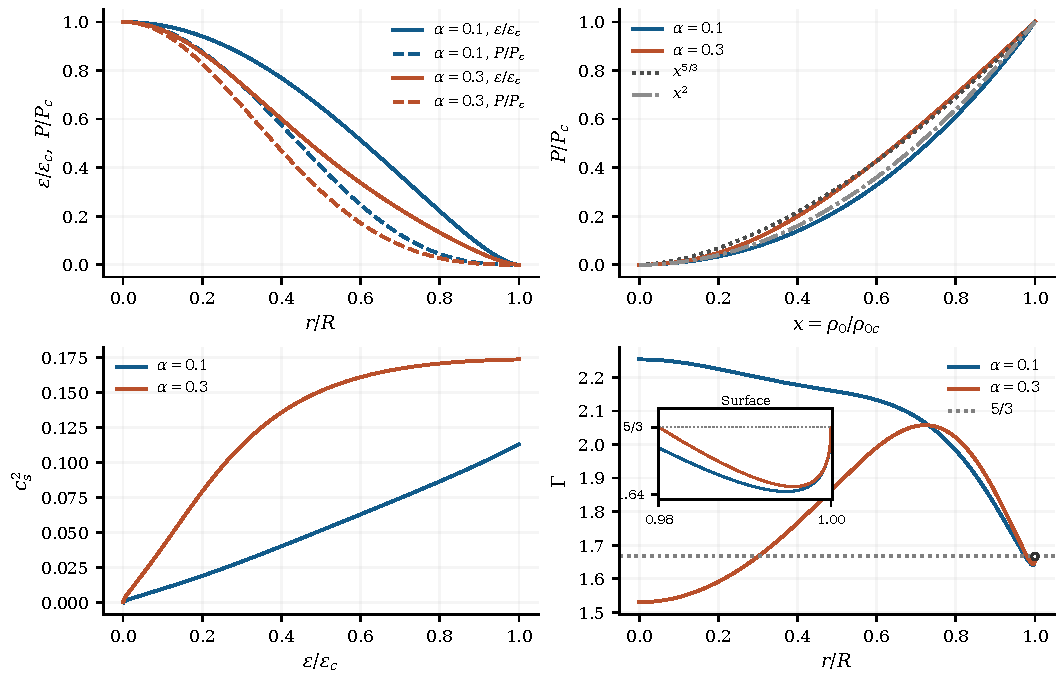
\includegraphics[width=\textwidth]{figures/background.pdf}
 \caption{Representative backgrounds at $\alpha=0.1$ and $0.3$. Top left: normalized density and pressure. Top right: the reconstructed EOS in terms of rest-mass density $\rho_0=m_bn$; the $x^{5/3}$ and $x^2$ curves are reference polytropic laws normalized at the centre, rather than separate stellar configurations. Bottom left: sound speed versus energy density. Bottom right: the adiabatic index. The inset resolves its shallow outer minimum and approach to $5/3$ from below. Interior points extend to $1-r/R=5\times10^{-9}$, and the endpoint is the analytical limit. \aiplotnote}
 \label{fig:background}
\end{figure*}

\begin{table}[t]
\centering
\caption{Representative dimensionless backgrounds, rounded to at most six significant figures.}
\label{tab:background}
\begin{tabular}{lrr}
\toprule
Quantity & $\alpha=0.1$ & $\alpha=0.3$\\
\midrule
$M/R$ & 0.0820771 & 0.15885\\
$8\pi R^2\varepsilon_c$ & 1.66214 & 4.65375\\
$8\pi R^2P_c$ & 0.0878642 & 0.596246\\
$(c_s^2)_c$ & 0.113126 & 0.173781\\
$\Gamma_c$ & 2.25315 & 1.53015\\
$\max(P/\varepsilon)$ & 0.0528613 & 0.12812\\
$\min f$ & 0.821231 & 0.649572\\
\bottomrule
\end{tabular}
\end{table}

On the sampled family, loss of monotone stiffening first appears near the centre. The central derivative $(c_s^2)_s(0)$ vanishes at $\alpha\simeq0.3151$, corresponding to $\mathcal C=M/R\simeq0.1624$. Beyond this point, the sound-speed maximum moves away from the centre. The maximum reaches unity only at $\alpha\simeq8.946$, $\mathcal C\simeq0.2745$, at $r/R\simeq0.30783$. Figure~\ref{fig:family} and Table~\ref{tab:limits} separate these restrictions from the radial-stability boundary calculated below.

\begin{figure*}[t]
 \centering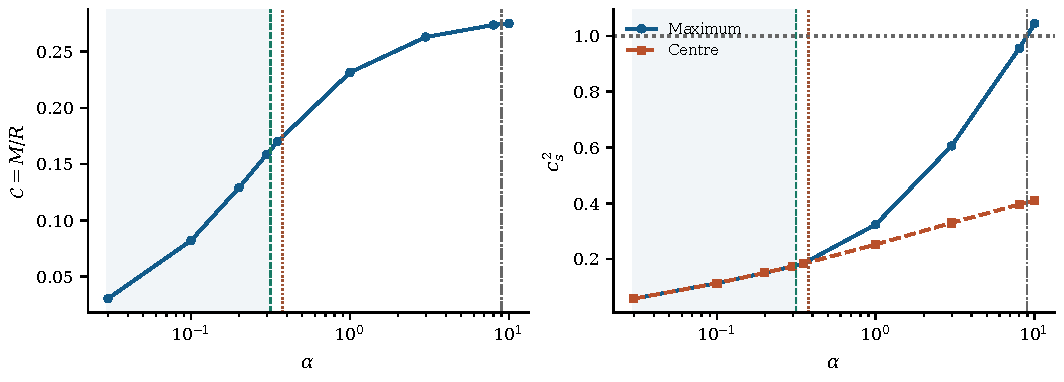
\includegraphics[width=\textwidth]{figures/family.pdf}
 \caption{Compactness and sound speed along the generating family. Points are evaluated configurations; connecting lines guide the eye. The shaded range extends to the numerical monotone-stiffening limit. Vertical lines indicate that limit (dashed), the radial-mode zero crossing (dotted), and the causal limit (dash-dotted). The thresholds are located by root-finding, with radial maximization for the causal bound, rather than inferred from the plotted markers. Changing $\alpha$ changes the EOS. \aiplotnote}
 \label{fig:family}
\end{figure*}

\begin{table}[t]
\centering
\caption{Numerically located boundaries of distinct properties.}
\label{tab:limits}
\begin{tabular}{lrr}
\toprule
Property lost & $\alpha$ & $\mathcal C$\\
\midrule
Monotone stiffening & 0.3151 & 0.1624\\
Radial stability & 0.3763 & 0.1751\\
Causality & 8.946 & 0.2745\\
\bottomrule
\end{tabular}
\end{table}

These boundaries are numerical determinations. In particular, the central-slope condition is supported by radial sampling rather than a validated global sign enclosure. The working examples $\alpha=0.1$ and $0.3$ lie within the sampled monotone-stiffening domain. The more compact part of the family remains useful for studying the separate failure mechanisms, but it does not satisfy all of the original physical conditions.

\subsection{Energy conditions and physical scale}
The sampled configurations through the causal boundary have $\varepsilon>0$, $P\ge0$ and $P\le\varepsilon$. These inequalities imply the weak, dominant and strong energy conditions for this perfect fluid. They are also well below the Buchdahl bound $\mathcal C<4/9$ for static isotropic spheres with nonincreasing density~\cite{buchdahlbound}. The causal-boundary model has $\max(P/\varepsilon)\simeq0.851$; failure of the dominant energy condition therefore does not set that boundary.

The free length scale permits a physical normalization without changing the dimensionless solution. At $R=12\,\mathrm{km}$, the masses for $\alpha=0.1$ and $0.3$ are approximately $0.667$ and $1.291\,M_\odot$. These examples illustrate relativistic compactness rather than a calibrated nuclear-matter EOS.

\subsection{Thermodynamic profiles}
The reconstruction also determines the rest-mass density $\rho_0=m_bn$ and the internal energy above rest mass. In $c=1$ units, define
\begin{align}
 h&=\Phi_b-\Phi=\ln(\mathcal H_b/m_b),\nonumber\\
 \Theta&=P/\rho_0,\qquad K_{\rm eff}=P/\rho_0^{5/3},\nonumber\\
 u_{\rm int}&=\frac{\varepsilon}{\rho_0}-1=e^h-1-\Theta.\label{eq:thermal}
\end{align}
Figure~\ref{fig:thermo} shows the rest-mass density, enthalpy and internal-energy profiles, together with $K_{\rm eff}$. The central enthalpies $\mathcal H_b/m_b$ are $1.10812$ and $1.33375$ for $\alpha=0.1$ and $0.3$. The variation of $K_{\rm eff}$ shows that the interior is not a global $5/3$ polytrope.

The quantity $\Theta$ is pressure per particle in rest-energy units. Its full radial profile is given in the supplement, without assigning a core temperature. A barotrope $\varepsilon(n)$ alone does not determine temperature or heat capacity: these require an entropy-dependent EOS. Likewise $\mathcal H_b$ is enthalpy, not generally the finite-entropy chemical potential. No Tolman thermal-equilibrium condition is imposed.

Keeping one additional surface term gives
\begin{align}
 E+\Pi&=e_3z^3[1+2z+O(z^2)],\nonumber\\
 \Pi&=\frac{e_3g_b}{5}z^5[1+\tfrac53z+O(z^2)].
\end{align}
Together with~\eqref{eq:n}, these imply
\begin{align}
 \Gamma&=\frac53-\frac59z+O(z^2),\label{eq:gaslimit}\\
 \Theta&=\frac{g_b}{5}z^2[1-\tfrac13z+O(z^2)],&
 \frac{u_{\rm int}}{\Theta}&\longrightarrow\frac32.\nonumber
\end{align}
The leading surface relations are those of a nonrelativistic monatomic gas: $\Gamma\to5/3$ and $u_{\rm int}/\Theta\to3/2$. They are compatible with either a hot isentropic ideal gas or a zero-temperature, noninteracting degenerate Fermi gas; these two interpretations cannot be distinguished by the barotrope alone. Only in the thermal ideal-gas interpretation does $P/(nk_{\rm B})$ become a temperature. In contrast, $\Gamma_c\simeq2.25315$ at $\alpha=0.1$ exceeds the stiffness of either free monatomic-gas description. Such an interior requires additional physics, for example interactions, and is not identified here with a specific microscopic material.

The approach of $\Gamma$ to $5/3$ is therefore from below. Its outer local minima occur at $r/R\simeq0.99475$ and $0.99564$, with $\Gamma\simeq1.64119$ and $1.64313$, respectively. For $\alpha=0.3$ this is not the global minimum, since $\Gamma_c$ is lower. The surface law and the outer rise in $K_{\rm eff}$ are genuine properties of the reconstructed EOS.

\begin{figure*}[t]
 \centering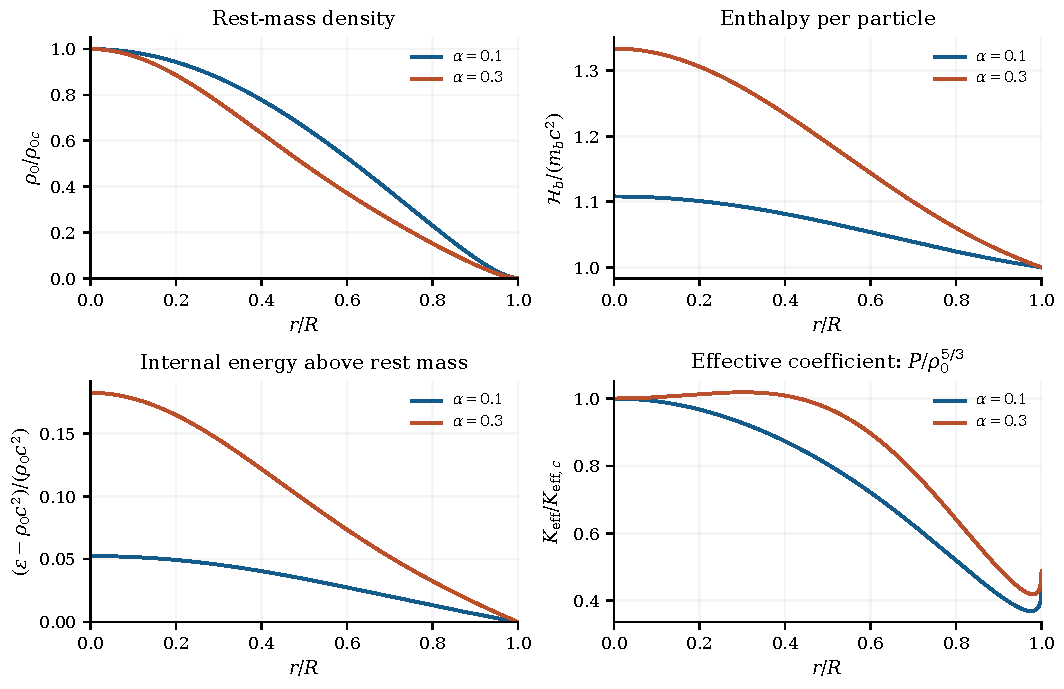
\includegraphics[width=\textwidth]{figures/thermodynamic_profiles.pdf}
 \caption{Thermodynamic profiles of the two representative configurations. Top left: rest-mass density normalized at the centre. Top right: enthalpy per particle, which tends to the rest-mass energy. Bottom left: internal energy above rest mass. Bottom right: $K_{\rm eff}=P/\rho_0^{5/3}$ normalized at the centre. Factors of $c$ are restored in the axis labels. All panels follow directly from the isentropic barotrope; none assigns a physical core temperature. \aiplotnote}
 \label{fig:thermo}
\end{figure*}

\section{Rotation through second order}
\subsection{Metric and exact first-order moment of inertia}
Write $\mathsf P_2=(3\cos^2\theta-1)/2$. The Hartle metric, expanded and retained through $O(\Omega^2)$, is
\begin{align}
 \dd\sigma^2={}&-e^{2\Phi}(1+2h_0+2h_2\mathsf P_2)\dd t^2\nonumber\\
 &+\frac1f\left[1+\frac{2(m_0+m_2\mathsf P_2)}{rf}\right]\dd r^2\nonumber\\
 &+r^2(1+2k_2\mathsf P_2)
 \left[\dd\theta^2+\sin^2\theta(\dd\phi-\omega\dd t)^2\right].
 \label{eq:hartlemetric}
\end{align}
The functions $h_0,h_2,m_0,m_2,k_2$ have order $\Omega^2$; $\omega$ has order $\Omega$. In~\eqref{eq:hartlemetric}, products beyond the retained order are discarded. The fluid rotates uniformly, $u^\mu=u^t(1,0,0,\Omega)$.

Matching $W$ to $\Omega-2J/r^3$ at $R=1$ gives
\begin{equation}
 \Omega=W_b+W'_b/3,\qquad J=W'_b/6.
\end{equation}
Using~\eqref{eq:F} and~\eqref{eq:norm},
\begin{equation}
 \boxed{\frac{I}{R^3}=\frac{8\alpha}{27(1+26\alpha/9)}},\qquad J=I\Omega.
 \label{eq:I}
\end{equation}
For example, $I/R^3=2/87$ at $\alpha=0.1$ and $1/21$ at $\alpha=0.3$. The rational values arise from the polynomial boundary data and their normalization.

\subsection{Interior equations and reconstruction}
Introduce
\begin{equation}
 q=\frac{m}{r^3},\quad g=\frac{\Phi'}r,\quad
 S=\frac{E+\Pi}{2},\quad \chi=\frac{S}{c_s^2}=-\frac{E_s}{g}.
\end{equation}
The last expression evaluates the removable surface limit without dividing two vanishing matter functions. Define the known rotational sources
\begin{align}
 \mathcal U&=\frac23s j^2W_s^2,&
 \mathcal V&=-\frac43j^2a_j W^2,\nonumber\\
 \mathcal T&=\frac13s e^{-2\Phi}W^2,&
 \mathcal T_s&=\frac{e^{-2\Phi}}3\left[(1-sg)W^2+2sWW_s\right].
 \label{eq:sources}
\end{align}
Regular variables are
\begin{equation}
 m_0=r^3\zeta,\qquad h_2=sX,\qquad v_2:=h_2+k_2=s^2Y.
\end{equation}
For fixed central density, the monopole equations are
\begin{align}
 2s\zeta_s+3\zeta&=\chi p_0+s(\mathcal U/2+\mathcal V),\label{eq:mono1}\\
 (p_0)_s&=-\frac{(1+s\Pi)\zeta}{2f^2}
       +a_j p_0+\frac{s\mathcal U}{4f}+\mathcal T_s,\label{eq:mono2}
\end{align}
with $\zeta(0)=p_0(0)=0$. The quadrupole satisfies
\begin{equation}
 2s\binom{X}{Y}_s=C_q\binom{X}{Y}+\boldsymbol d_q,
 \label{eq:quad}
\end{equation}
where
\begin{align}
 C_q&=\begin{pmatrix}
 -2-2sg+(S-2q)/(fg)&-2/(fg)\\
 -2g&-4
 \end{pmatrix},\label{eq:Cq}\\
 \boldsymbol d_q&=\binom{s^2g(\mathcal U+\mathcal V)+(\mathcal V-\mathcal U)/(2fg)}
 {(1+sg)(\mathcal U+\mathcal V)}.\label{eq:dq}
\end{align}
Let $g_c=g(0)$. One regular particular solution and the regular homogeneous solution have central data
\begin{equation}
 \binom{X^p}{Y^p}_{\!0}=\binom{0}{\mathcal V_c/4},\qquad
 \binom{X^h}{Y^h}_{\!0}=\binom{1}{-g_c/2}.
\end{equation}
The interior solution is $(X,Y)=(X^p,Y^p)+c_q(X^h,Y^h)$. The other functions follow algebraically:
\begin{align}
 h_0&=c_h-p_0+\mathcal T,& k_2&=v_2-h_2,\nonumber\\
 m_2&=rf[-h_2+s^2(\mathcal U+\mathcal V)],&p_2&=-h_2-\mathcal T,\label{eq:reconstruct}\\
 \delta P&=(\varepsilon+P)(p_0+p_2\mathsf P_2),&
 \delta\varepsilon&=\delta P/c_s^2.\nonumber
\end{align}
Here $p_0,p_2$ are dimensionless enthalpy perturbations, not background pressures. Equations~\eqref{eq:mono1}--\eqref{eq:reconstruct} are the standard second-order Einstein-fluid equations in centre-regular variables. Appendix~\ref{app:volterra} specifies their regular solutions by a convergent Volterra series.

\subsection{Exterior solution and matching constants}
Outside the fluid, use $f=e^{2\Phi}=1-2M/r$, $\omega=2J/r^3$ and $x=r/M-1$. Define the elementary vacuum functions
\begin{align}
 \mathcal Q(x)&=\frac32(x^2-1)\ln\frac{x+1}{x-1}
                -\frac{3x^3-5x}{x^2-1},\label{eq:Qvac}\\
 \mathcal V_q(x)&=2\left[\frac{3x^2-2}{x^2-1}
                  -\frac32x\ln\frac{x+1}{x-1}\right].
\end{align}
The exterior functions in the same metric convention are
\begin{align}
 m_0^+&=\delta M-J^2/r^3,&h_0^+&=-\frac{m_0^+}{r-2M},\nonumber\\
 h_2^+&=J^2\left(\frac1{Mr^3}+\frac1{r^4}\right)+K\mathcal Q(x),\nonumber\\
 v_2^+&=-J^2/r^4+K\mathcal V_q(x),& k_2^+&=v_2^+-h_2^+,\label{eq:exterior}\\
 m_2^+&=(r-2M)\left[-h_2^++\frac{6J^2}{r^4}\right].\nonumber
\end{align}
At $r=1$, the matching constants are determined by
\begin{align}
 \delta M&=m_0(1)+J^2,\label{eq:dM}\\
 c_h&=h_0^+(1)+p_0(1)-\mathcal T(1),\nonumber\\
 \begin{pmatrix}h_2^h(1)&-\mathcal Q(x_b)\\
 v_2^h(1)&-\mathcal V_q(x_b)\end{pmatrix}\binom{c_q}{K}
 &=\binom{J^2(1/M+1)-h_2^p(1)}{-J^2-v_2^p(1)},\label{eq:match}
\end{align}
where $x_b=1/M-1$. Both pressure and density vanish at the surface, so there is no surface-density contribution to~\eqref{eq:dM} of the kind identified in the revised matching treatment~\cite{reinavera}. The solutions match without a surface stress layer.

The total mass is $M+\delta M$, and the mass quadrupole in the convention that an oblate star has $Q<0$ is
\begin{equation}
 Q=-\frac{J^2}{M}-\frac85KM^3.
 \label{eq:quadrupole}
\end{equation}
The coefficient $K$ is determined by the interior. It is not fixed to its Kerr value.

\subsection{Surface deformation and geometric shape}
In the radial coordinate of~\eqref{eq:hartlemetric},
\begin{align}
 r_{\rm surf}&=1+\xi_0+\xi_2\mathsf P_2,\nonumber\\
 \xi_0&=\frac{p_0(1)}{\Phi'(1)},&
 \xi_2&=\frac{-h_2(1)-\mathcal T(1)}{\Phi'(1)}.
 \label{eq:surface}
\end{align}
An Eulerian expansion of the matter variables is nonuniform arbitrarily close to this displaced zero-density boundary. A density-surface label $\bar r$ resolves the issue:
\begin{equation}
 r=\bar r+\xi(\bar r,\theta),\qquad
 \xi=\frac{p_0+p_2\mathsf P_2}{\Phi'}.
 \label{eq:lagrange}
\end{equation}
Pulling back the metric with
$\dd r=(1+\xi_{,\bar r})\dd\bar r+\xi_{,\theta}\dd\theta$
gives a surface at $\bar r=1$. Since $\delta P+P'\xi=0$, the matter variables are their background functions of $\bar r$ through the retained order. This change of coordinates adds no physical shell.

To describe shape without identifying coordinate radii with proper distances, consider the induced metric on a constant-$t$ surface section. Restoring $R$, let
\begin{equation}
 d_0=\xi_0/R,\qquad d_2=\xi_2/R+k_2(R).
\end{equation}
Its two-metric is $R^2(1+2d_0+2d_2\mathsf P_2)\dd\Omega_2^2$ through $O(\Omega^2)$. An axisymmetric Euclidean embedding to this order has meridian
\begin{align}
 \varpi_{\rm emb}/R&=(1+d_0+d_2\mathsf P_2)\sin\theta,\nonumber\\
 Z_{\rm emb}/R&=(1+d_0-d_2/2)\cos\theta
                  +\tfrac32d_2\cos^3\theta.\label{eq:embedding}
\end{align}
The flattening of this embedded surface is $-3d_2/2+O(\Omega^4)$. It refers to the specified spatial section, not a unique relativistic definition of a polar radius.

\begin{figure*}[t]
 \centering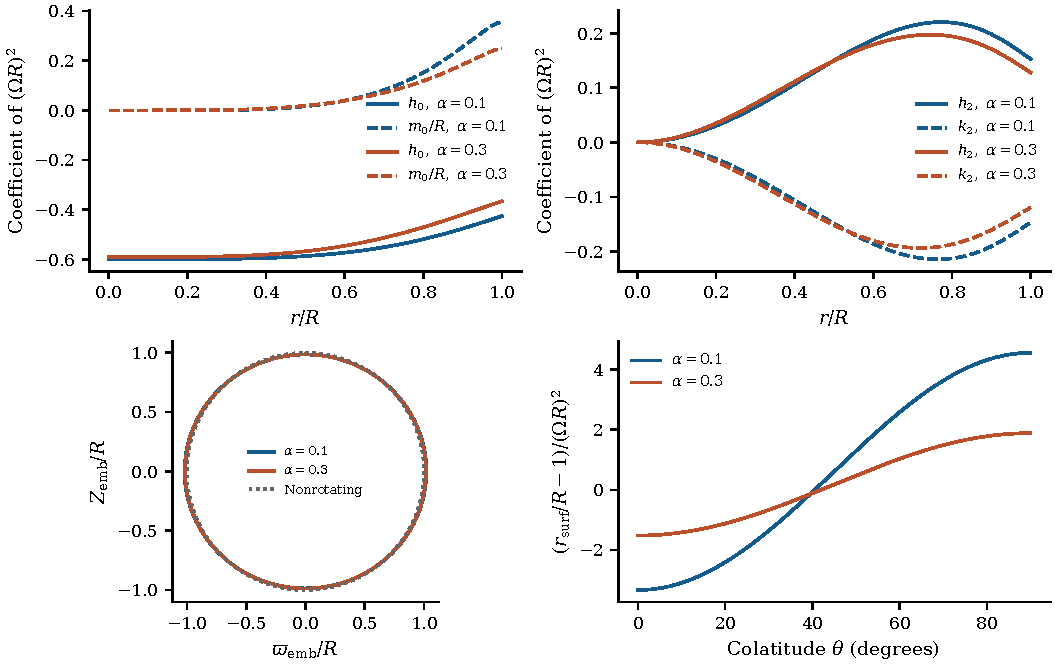
\includegraphics[width=\textwidth]{figures/rotation.pdf}
 \caption{Second-order rotation at fixed central density. Top: monopole and quadrupole metric coefficients divided by $(\Omega R)^2$. Bottom left: the embedded surface~\eqref{eq:embedding} at $\Omega^2R^3/M=0.05$, with the nonrotating circle for reference. Bottom right: the coordinate surface displacement~\eqref{eq:surface}, shown as its coefficient of $(\Omega R)^2$. The two surface panels therefore represent distinct, explicitly defined notions of shape. \aiplotnote}
 \label{fig:rotation}
\end{figure*}

For $\alpha=0.1$, the coordinate surface is
\begin{align}
 \frac{r_{\rm surf}}R={}&1+(\Omega R)^2
       (1.92403-5.25122\mathsf P_2)\nonumber\\
       &+O(\Omega^4R^4),
\end{align}
and $k_2(R)=-0.146681(\Omega R)^2$. The corresponding flattening is $8.09685(\Omega R)^2$.

\section{Multipoles and tides}
\subsection{Tidal response and I--Love--Q relations}
The tidal Love number is denoted $k_2^{\rm tid}$ to distinguish it from the rotational metric function $k_2(r)$. Following Hinderer and the published erratum~\cite{hinderer,hinderererratum}, integrate the static tidal variable $y=rH_{\rm tid}'/H_{\rm tid}$, with $y(0)=2$. In the present variables,
\begin{align}
 2s y_s&=-y^2-yF_t-Q_t,\nonumber\\
 F_t&=\frac{1-s(E-\Pi)/2}{f},\label{eq:tide}\\
 Q_t&=\frac{s(5E+9\Pi-2E_s/g)/2-6}{f}-4s^2g^2.\nonumber
\end{align}
Let $y_b=y(1)$, $\mathcal C=M/R$ and $A_t=2+2\mathcal C(y_b-1)-y_b$. The exterior match gives
\begin{equation}
 k_2^{\rm tid}=\frac{8\mathcal C^5(1-2\mathcal C)^2 A_t}{5D_t},
\end{equation}
where
\begin{align}
 D_t={}&2\mathcal C[6-3y_b+3\mathcal C(5y_b-8)]\nonumber\\
 &+4\mathcal C^3[13-11y_b+\mathcal C(3y_b-2)
                         +2\mathcal C^2(1+y_b)]\nonumber\\
 &+3(1-2\mathcal C)^2 A_t\ln(1-2\mathcal C).
\end{align}
There is no finite-density surface jump. As an independent check, $y_b$ is also obtained from the regular homogeneous quadrupole solution in~\eqref{eq:quad}; the two determinations agree within $1.9\times10^{-11}$ on the sampled models.

The dimensionless response quantities are
\begin{equation}
 \bar I=\frac{I}{M^3},\qquad
 \bar Q=-\frac{QM}{J^2},\qquad
 \Lambda=\frac{2k_2^{\rm tid}}{3\mathcal C^5}.
 \label{eq:dimensionless}
\end{equation}
Table~\ref{tab:response} reports selected members. Figure~\ref{fig:universal} compares them with the empirical fits of Yagi and Yunes~\cite{yagiscience,yagiyunes}. The residual is the calculated $\bar I$ divided by the fitted value, minus one. At $\alpha=0.1$, $\bar I=41.5762$, $\bar Q=18.3436$, and the I--Q residual is $+0.0792\%$. At $\alpha=0.3$, it is $-2.8258\%$. The corresponding I--Love residuals are $+1.3448\%$ and $-0.4071\%$.

\begin{table*}[t]
\centering
\caption{Rotational and tidal response along the family. The mass correction holds central density fixed; $Q<0$ denotes an oblate configuration. The last two rows lie outside the monotone-stiffening domain and are radially unstable.}
\label{tab:response}
\begin{tabular}{rrrrrrr}
\toprule
$\alpha$ & $\mathcal C$ & $I/R^3$ & $Q/(\Omega^2R^5)$ & $\delta M/(\Omega^2R^3)$ & $k_2^{\rm tid}$ & $\Lambda$\\
\midrule
0.1 & 0.0820771 & 0.0229885 & -0.118109 & 0.356257 & 0.128635 & 23022.8\\
0.2 & 0.128965 & 0.0375587 & -0.0915831 & 0.290259 & 0.0777477 & 1452.9\\
0.3 & 0.15885 & 0.0476191 & -0.0778688 & 0.251477 & 0.0539808 & 355.808\\
1.0 & 0.23158 & 0.0761905 & -0.0560093 & 0.168403 & 0.0181209 & 18.1378\\
8.0 & 0.273814 & 0.0983103 & -0.0531159 & 0.128961 & 0.00806212 & 3.4920\\
\bottomrule
\end{tabular}
\end{table*}

\begin{figure*}[t]
 \centering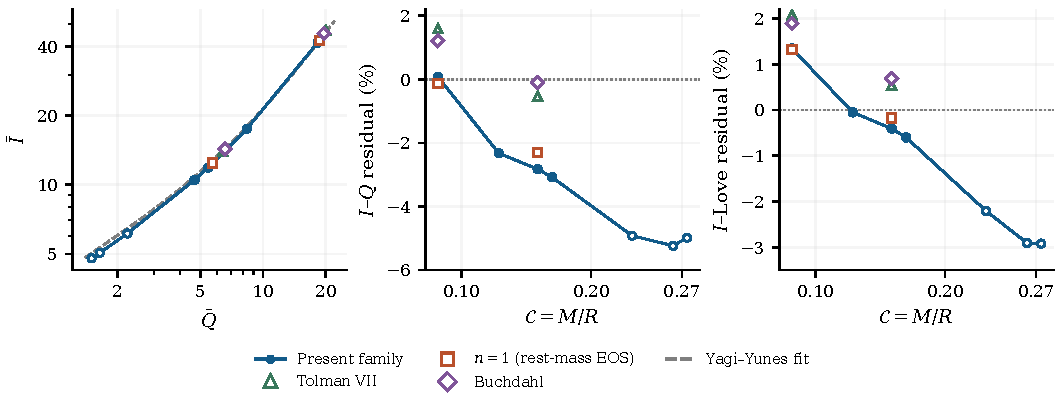
\includegraphics[width=\textwidth]{figures/universal.pdf}
 \caption{Comparison with the Yagi--Yunes fits~\cite{yagiyunes}. Left: I--Q relation. Centre and right: residuals $\bar I/\bar I_{\rm fit}-1$ for I--Q and I--Love. Reference models are evaluated at the two compactnesses of Table~\ref{tab:background}; the index-one reference uses rest-mass density in its EOS. Family points cover $0.1\le\alpha\le8$, with connecting segments as guides. Hollow blue circles denote the radially unstable sampled members $\alpha=1,3,8$; the hollow reference-model symbols distinguish those models only. The fits characterize response phenomenology and are not tests of the field equations. \aiplotnote}
 \label{fig:universal}
\end{figure*}

The close agreement at one parameter value is not uniform across the family. At still lower compactness the polynomial fit is extrapolated beyond the range relevant to the main examples, and its residual grows substantially. We therefore use the fits as comparisons rather than as constraints or correctness criteria.

\subsection{Comparison at equal compactness}
Three reference models are computed at the two compactnesses of Table~\ref{tab:background}. Tolman VII has
\begin{equation}
 \varepsilon(r)=\varepsilon_c(1-r^2/R^2),
 \qquad 8\pi R^2\varepsilon_c=15\mathcal C.
\end{equation}
Buchdahl's gaseous solution~\cite{buchdahlgas} has
\begin{equation}
 \varepsilon=12\sqrt{P_*P}-5P,
\end{equation}
where $P_*>0$ fixes the scale. The relativistic index-one polytrope is specified thermodynamically by
\begin{equation}
 P=K_{\rm p}\rho_0^2,\qquad \varepsilon=\rho_0+P,
 \qquad \rho_0=m_bn.
\end{equation}
The last expression follows from the first law for an isentropic gas and avoids identifying total energy density with rest-mass density. Each reference star is obtained from TOV and evaluated with the same dragging, quadrupole and tidal equations and the same sign convention for $Q$.

\begin{table*}[t]
\centering
\caption{Models compared at equal compactness. Scale-independent quantities are quoted to five significant figures. All entries are recomputed in a common convention.}
\label{tab:comparison}
\begin{tabular}{llrrrr}
\toprule
$\mathcal C$ & Model & $I/(MR^2)$ & $\bar Q$ & $k_2^{\rm tid}$ & $(c_s^2)_c$\\
\midrule
0.0820771 & Present, $\alpha=0.1$ & 0.28008 & 18.344 & 0.12864 & 0.11313\\
 & Tolman VII & 0.31583 & 20.060 & 0.18291 & 0.12405\\
 & Index-one polytrope & 0.28601 & 18.710 & 0.13740 & 0.096938\\
 & Buchdahl gas & 0.30673 & 19.631 & 0.16795 & 0.13920\\
\midrule
0.15885 & Present, $\alpha=0.3$ & 0.29977 & 5.4549 & 0.053981 & 0.17378\\
 & Tolman VII & 0.35274 & 6.4241 & 0.096468 & 0.30737\\
 & Index-one polytrope & 0.31398 & 5.7294 & 0.063974 & 0.23063\\
 & Buchdahl gas & 0.36179 & 6.5788 & 0.10530 & 0.77205\\
\bottomrule
\end{tabular}
\end{table*}

At either compactness, the present family has a smaller $I/(MR^2)$ and tidal response than these references, with the index-one polytrope the closest of the three. At $\mathcal C\simeq0.15885$, the difference in $k_2^{\rm tid}$ from Tolman VII is about $44\%$, while the dimensionless quadrupoles differ by about $15\%$. Equal compactness therefore does not remove the effect of density stratification. In Fig.~\ref{fig:universal}, the I--Q residual at this compactness is $-2.31\%$ for the index-one polytrope and $-0.54\%$ for Tolman VII, compared with $-2.83\%$ for the present family. The reference points place the family's deviations in context. The models also differ in their surface law: the three reference constructions have an index-one, $P\propto n^2$, low-density limit, whereas the present family has $P\propto n^{5/3}$.

\subsection{Mass correction at fixed baryon number}
The monopole calculation above fixes central density. To compare a rotating star with the same total particle number, define $M_b=m_bN_b$. For uniformly rotating equilibria at fixed EOS, composition and entropy per particle, the first law is~\cite{bardeen}
\begin{equation}
 \dd M=\Omega\,\dd J+\mathcal H_\infty\,\dd N_b.
 \label{eq:firstlaw}
\end{equation}
At the nonrotating configuration, $\mathcal H_\infty=m_b\sqrt{f_b}$. Write $M=M_0+M_2\Omega^2+O(\Omega^4)$, $M_b=M_{b0}+B_2\Omega^2+O(\Omega^4)$, and $J=I\Omega+O(\Omega^3)$. Equation~\eqref{eq:firstlaw} gives
\begin{equation}
 M_2=\frac I2+\sqrt{f_b}\,B_2,
 \qquad
 \left.\delta M\right|_{N_b}=\frac12I\Omega^2+O(\Omega^4).
 \label{eq:fixedN}
\end{equation}
Here $\mathcal H_\infty$ is the redshifted enthalpy per particle, constant in an isentropic equilibrium. Equation~\eqref{eq:fixedN} is a general first-law identity for a regular fixed-baryon sequence, not a special property of this family. Its agreement with independently integrated monopole and baryon corrections tests the calculation. The relevant variations keep the EOS fixed; they are not derivatives along the $\alpha$-family.

The independently integrated particle-number correction is
\begin{align}
 \delta M_b=4\pi\int_0^R\frac{r^2\rho_0}{\sqrt f}
 \left[\frac{m_0}{rf}+\frac{r^2e^{-2\Phi}W^2}{3}
                  +\frac{p_0}{c_s^2}\right]\dd r,
 \label{eq:baryon}
\end{align}
with $\rho_0=e^\Phi(\varepsilon+P)/\sqrt{f_b}$. The density vanishes at the surface, eliminating a boundary-displacement term. The integrand remains integrable despite the factor $1/c_s^2$.

For $\alpha=0.1$, $B_2/R^3=0.377101$ and $M_2/R^3=0.356257$, whereas the fixed-baryon coefficient is $0.0114943$. At $\alpha=0.3$, these values are $0.275622$, $0.251477$, and $0.0238095$. Using unrounded data, the residual in the first identity of~\eqref{eq:fixedN} is below $2.4\times10^{-11}$ in dimensionless units on the sampled family.

Away from a turning point, the full fixed-baryon monopole follows by adding the background derivative at fixed EOS, with
\begin{equation}
 \frac{\delta E_c}{\Omega^2}=
 \frac{I/2-M_2}{(\partial M/\partial E_c)_{\rm EOS}}.
\end{equation}
The quadrupole at order $\Omega^2$ is unaffected by this order-$\Omega^2$ shift of background. Near a turning point the denominator becomes small, so the central-density shift imposes an additional restriction on the perturbative regime.

\section{Stability and rotation scale}
\subsection{Sequences at fixed EOS}
For each reference configuration, reconstruct one EOS on the density range occupied by that star and vary its central enthalpy
\begin{equation}
 h=\int_0^P\frac{\dd\widetilde P}{\varepsilon(\widetilde P)+\widetilde P}
   =\Phi_b-\Phi.
\end{equation}
The sequences in Fig.~\ref{fig:stability} use $0.002\le h_c/h_{c,\rm ref}\le1$. They therefore require no high-density extrapolation. The reference stars are recovered independently by TOV integration. A decreasing mass beyond a maximum is a warning of instability; turning-point arguments must be applied to these fixed-EOS sequences rather than the generating family~\cite{btm,fis}.

\subsection{Radial pulsations}
We also calculate the nonrotating radial modes. For radial displacement $\xi_r$ and $Z_r=r^2e^{-\Phi}\xi_r$, the Sturm--Liouville equation is~\cite{chandra1964,btm}
\begin{equation}
 (\mathcal P_r Z_r')'+(\mathcal Q_r+\sigma^2\mathcal W_r)Z_r=0,
\end{equation}
where $e^{2\lambda_r}=1/f$ and
\begin{align}
 \mathcal P_r&=\frac{e^{\lambda_r+3\Phi}}{r^2}\Gamma P,\nonumber\\
 \mathcal Q_r&=\frac{e^{\lambda_r+3\Phi}}{r^2}
 \left[\frac{(P')^2}{\varepsilon+P}-\frac{4P'}r
       -8\pi P(\varepsilon+P)e^{2\lambda_r}\right],\label{eq:radial}\\
 \mathcal W_r&=\frac{e^{3\lambda_r+\Phi}}{r^2}(\varepsilon+P).\nonumber
\end{align}
The boundary conditions are $Z_r=O(r^3)$ at the centre and $\mathcal P_rZ_r'\to0$ at the surface. The adiabatic derivative is the equilibrium EOS derivative, consistent with the isentropic model.

A Rayleigh--Ritz discretization uses the regular basis $r^3\mathsf P_k(2r^2-1)$ with 8, 16 and 24 functions. Table~\ref{tab:stability} gives the fundamental squared frequency and an independent fixed-EOS mass derivative. For the low-$\alpha$ examples, the fundamental value changes by less than $2\times10^{-9}$ between the 8- and 24-function calculations. The 16- to 24-function change is a few $10^{-12}$.

\begin{table}[t]
\centering
\caption{Nonrotating stability diagnostics in $R=1$ units; $E_c=8\pi\varepsilon_c$.}
\label{tab:stability}
\begin{tabular}{rrr}
\toprule
$\alpha$ & $(\partial M/\partial E_c)_{\rm EOS}$ & $\sigma_0^2R^2$\\
\midrule
0.1 & $+0.0406462$ & $+0.243925$\\
0.2 & $+0.0110838$ & $+0.174258$\\
0.3 & $+0.0025823$ & $+0.0715395$\\
0.3151 & $+0.0019104$ & $+0.0566943$\\
1 & $-0.0019987$ & $-0.317468$\\
8 & $-0.0000665$ & $\simeq-0.576$\\
\bottomrule
\end{tabular}
\end{table}

\begin{figure*}[t]
 \centering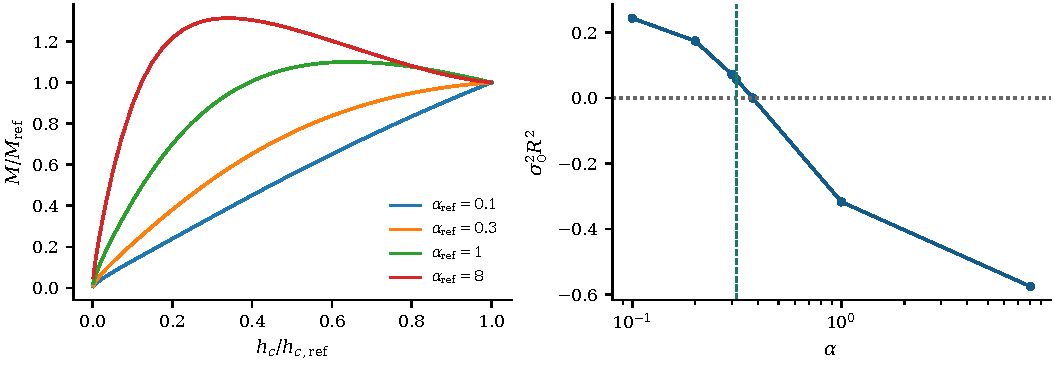
\includegraphics[width=\textwidth]{figures/stability.pdf}
 \caption{Left: TOV sequences, each calculated with the single EOS reconstructed from its labelled reference configuration. The reference model is at the right endpoint of each curve. Right: fundamental nonrotating radial-mode eigenvalues along the generating family, with connecting lines as guides. The dashed line marks the monotone-stiffening boundary. The radial zero crossing occurs later, at $\alpha\simeq0.3763$. \aiplotnote}
 \label{fig:stability}
\end{figure*}

The fundamental frequency crosses zero near $\alpha=0.3763$, $\mathcal C=0.1751$. Independently, the fixed-EOS mass derivative at that reference model approaches zero as its finite-difference step is reduced. Thus the numerical radial-stability boundary lies above the monotone-stiffening boundary. Positive Ritz eigenvalues are upper bounds rather than certified positive lower bounds; their convergence and agreement with the sequence calculation provide numerical stability evidence. The negative values at $\alpha=1$ and $8$ identify unstable backgrounds. The onset at $\mathcal C\simeq0.1751$ is consistent with core softening across the generating family: $\Gamma_c$ decreases from $2.25315$ at $\alpha=0.1$ to $1.53015$ at $\alpha=0.3$. This reduces pressure support against relativistic self-gravity even while $c_s^2$ remains causal. Since the EOS changes with $\alpha$, this is a trend between different materials, not a fixed-EOS evolutionary sequence; the full radial eigenproblem, rather than $\Gamma_c$ alone, determines the stability boundary.

\subsection{Rotation scale}
The slow-rotation parameter is
\begin{equation}
 \eta_{\rm rot}=\frac{\Omega^2R^3}{M}\ll1.
\end{equation}
It must be accompanied by small actual metric and surface perturbations. A useful frequency scale, restoring $c$, is
\begin{equation}
 f_{\rm dyn}=\frac{c}{2\pi R}\sqrt{\mathcal C}.
\end{equation}
This is the Schwarzschild circular-orbit frequency at the unperturbed surface, measured at infinity. At $R=12\,\mathrm{km}$ it is about $1139$ and $1585\,\mathrm{Hz}$ for the two examples. Taking $\eta_{\rm rot}=0.01$ gives spin frequencies of about $114$ and $158\,\mathrm{Hz}$. These values characterize a slow-rotation scale; a rotating mass-shedding limit requires the deformed configuration and is not determined by this estimate.

\section{Validation}\label{sec:validation}
\subsection{Computational provenance}
OpenAI ChatGPT and Codex assisted the development of the construction and derivations, the generation and debugging of numerical and plotting code, and the interpretation of the calculated diagnostics. The numerical results were obtained by executing the supplied Python programs, rather than treating language-model predictions as data. The checks below include alternative formulations of the field equations, convergence studies and external published benchmarks. They document computational validation; agreement between AI-assisted implementations is not by itself independent human verification. The use of these tools in manuscript preparation is disclosed in the acknowledgments.

\subsection{Internal consistency}
The background is evaluated both from its quadratures and from a centre-regular isotropy equation given in Appendix~\ref{app:centre}. At $\alpha=0.1$, representative comparisons agree at approximately $10^{-13}$. Near the surface, pressure is evaluated by its hydrostatic integral when needed, avoiding subtraction of order-$z^3$ terms to obtain an order-$z^5$ result. The fixed-EOS TOV reconstruction recovers the reference mass and radius to better than about $6\times10^{-11}$ for $\alpha\le1$; the errors remain below a few $10^{-9}$ at $\alpha=8$.

The quadrupole matching system~\eqref{eq:match} is solved after scaling each column to unit Euclidean norm. At $\alpha=0.1$, the matrix condition number decreases from about $2661$ to $12.47$. The small unscaled determinant mainly reflects the amplitude of the decaying vacuum basis, rather than an intrinsically singular match. Cancellation in~\eqref{eq:Qvac} at small compactness is avoided using the convergent expansions, for $x>1$,
\begin{align}
 \mathcal Q(x)&=\sum_{k=1}^{\infty}
 \frac{8k(k+2)}{(2k+1)(2k+3)}x^{-2k-1},\nonumber\\
 \mathcal V_q(x)&=\sum_{k=1}^{\infty}
 \frac{4(k-1)}{2k+1}x^{-2k}.
\end{align}
The 80 retained terms suffice for the sampled exterior matching points.

The Volterra representation and direct integration of the second-order equations agree to roughly ten significant digits for the $\alpha=0.1$ benchmark. Independent tidal and baryon-number calculations provide the additional checks reported above. The common comparison solver reproduces the present family's algebraic $I$ and its separately calculated $Q$ and $k_2^{\rm tid}$; these are internal consistency checks. For Buchdahl's model, the integrated compactness also agrees with its exact central-enthalpy relation $\mathcal C=(1-e^{-2h_c})/2$ to about $2\times10^{-11}$.

\subsection{Published rotational benchmarks}
To test the exterior matching that determines $K$, we apply the comparison solver to two published benchmarks. First, the exact uniform-density Schwarzschild interior reproduces Table~I of Chandrasekhar and Miller~\cite{cm}. With $R_S=2M$, their inertia column is $I/R_S^3$ and their positive-oblate quadrupole column is $|Q|/(J^2/R_S)$; conversion to~\eqref{eq:dimensionless} multiplies the former by eight and divides the latter by two. At $\mathcal C=0.1,1/6,1/4$, the largest relative differences are $0.037\%$ in $\bar I$ and $0.016\%$ in $\bar Q$. These comparisons concern the historical numerical values, rather than exact agreement with every last printed digit. Only rotational quantities are used: a Love-number calculation for a homogeneous model would additionally require its finite-density surface jump.

Second, we reproduce the $n=1$ polytropic curves in Figs.~6 and 7 of Yagi and Yunes~\cite{yagiyunes}. Their convention is $P=K\varepsilon^2$, distinct from the rest-mass polytrope in Table~\ref{tab:comparison}. Table~\ref{tab:external} compares three vertices extracted from the authors' original vector figures. The largest differences are $0.044\%$ in $\bar I$ and $0.035\%$ in $\bar Q$, within a conservative $0.16$--$0.21\%$ graphical-resolution allowance propagated from both coordinate directions. This is a comparison with published model curves, not with a universal-relation fit.

\begin{table*}[t]
\centering
\caption{External $n=1$ benchmark, $P=K\varepsilon^2$. Published values are digitized from the original vector curves of Ref.~\cite{yagiyunes}; values are displayed to at most six significant figures, with the extraction coordinates and unrounded values retained in the data archive. Differences are calculated/digitized minus one.}
\label{tab:external}
\begin{tabular}{rrrrrrr}
\toprule
$\mathcal C$ & $\bar I_{\rm pub}$ & $\bar I_{\rm calc}$ & Difference (\%) & $\bar Q_{\rm pub}$ & $\bar Q_{\rm calc}$ & Difference (\%)\\
\midrule
0.0775627 & 47.8822 & 47.8893 & $+0.01488$ & 20.5596 & 20.5543 & $-0.02598$\\
0.154091 & 13.5628 & 13.5642 & $+0.01031$ & 6.28988 & 6.28803 & $-0.02951$\\
0.200056 & 8.69298 & 8.68917 & $-0.04380$ & 3.57675 & 3.57551 & $-0.03448$\\
\bottomrule
\end{tabular}
\end{table*}

Reducing the central cutoff from $s=10^{-7}$ to $10^{-8}$ changes the selected benchmark responses by less than $2\times10^{-11}$ relatively. Applied to our two principal backgrounds, this externally tested solver recovers $I$ within $5.1\times10^{-11}$ and $Q$ within $4.5\times10^{-10}$ relative to the main implementation. The external tests therefore supplement, rather than duplicate, the internal consistency checks.

\subsection{Einstein-tensor residuals}
Numerical differentiation of~\eqref{eq:hartlemetric} supplies its Einstein tensor independently of the perturbation ODEs. At $r/R=0.55$, $\theta=1.1$, and $\alpha=0.3$, halving $\Omega R$ from $0.04$ to $0.02$ reduces the largest diagonal Einstein--matter residual from $3.06\times10^{-6}$ to $1.88\times10^{-7}$, approximately the expected factor of 16. The $t\phi$ residual decreases from $3.19\times10^{-5}$ to $3.99\times10^{-6}$, a factor of 8. These are the expected $O(\Omega^4)$ even-parity and $O(\Omega^3)$ odd-parity remainders; the nonrotating differentiation noise is about $10^{-8}$. The analytical perturbative construction rests on the reduced Einstein-fluid equations, while these checks test their implementation and reconstruction.

\section{Conclusions}
The prescribed dragging profile yields a continuously stratified relativistic fluid with a finite $P\propto n^{5/3}$ surface, exact static quadratures and an algebraic moment of inertia. The second-order Hartle--Thorne construction determines the rotational interior, the exterior quadrupole and the displaced surface. Published homogeneous-star and polytropic benchmarks support the rotational matching, while the general fixed-baryon first-law identity provides a separate monopole check.

The family separates causality, monotone stiffening and radial stability: increasing the parameter loses these properties at different compactnesses. The two principal examples have positive, converged radial-mode estimates and satisfy the sampled physical conditions. Their thermodynamic profiles recover the adiabatic gas surface continuously, and comparisons at equal compactness reveal the remaining influence of density stratification on rotational and tidal response.

The background and first-order solution are explicit in quadratures and algebraic functions. The second-order interior has a convergent integral representation, but no finite expression in standard special functions has been obtained. Within that scope, the family supplies a reproducible full-GR slow-rotation benchmark with a smooth gaseous surface.

\section*{Acknowledgments and AI disclosure}
OpenAI ChatGPT and Codex were used extensively for analytical suggestions and derivations, numerical-code development and debugging, literature discovery and checking, interpretation of results, figure-program development, and drafting and revising this manuscript. The assistance extended beyond language editing. All plots were rendered by Python from the recorded calculations and source data. Computational validation is described in Sec.~\ref{sec:validation} and in the supplement. Responsibility for the scientific claims, interpretation, references and final submitted text rests with the human author; no AI system is credited as an author.

\section*{Data and code availability}
The numerical data underlying the tables and figures, calculation and plotting programs, source-provenance records, and LaTeX sources are supplied in the accompanying reproducibility archive. The supplement documents the external benchmarks and near-surface checks. Unrounded numerical results are retained in the archive. The published comparison papers remain available from the cited sources.

\ifdefined\appendices\appendices\else\appendix\fi
\section{Regular centre evaluation}
\label{app:centre}
For numerical evaluation set $u=(f-1)/s$. Equation~\eqref{eq:isotropy} becomes
\begin{align}
 2s u_{ss}+(5-6sa_j)u_s
 &+[-6a_j+4s(a_j^2-a_{j,s})]u\nonumber\\
 &+4(a_j^2-a_{j,s})=0.
\end{align}
A regular particular solution and homogeneous solution determine $u$, with its central constant fixed by $3u(1)+2u_s(1)=0$. Write
\begin{align}
 f&=1+c_f s+u_1s^2+u_2s^3+\cdots,\nonumber\\
 a_j&=a_0+a_1s+a_2s^2+\cdots.
\end{align}
The coefficients needed for central sound-speed derivatives are
\begin{align}
 a_0&=-35\alpha/8,\nonumber\\
 a_1&=35\alpha/16+735\alpha^2/32,\nonumber\\
 a_2&=385\alpha/64-1085\alpha^2/64-15435\alpha^3/128,\\
 u_1&=[6a_0c_f-4(a_0^2-a_1)]/5,\nonumber\\
 u_2&=[12a_0u_1+(10a_1-4a_0^2)c_f-8a_0a_1+8a_2]/14.
\end{align}
With $E=E_c+e_{c1}s+e_{c2}s^2+\cdots$ and $\Pi=\Pi_c+p_{c1}s+p_{c2}s^2+\cdots$,
\begin{align}
 E_c&=-3c_f,&\Pi_c&=3c_f-4a_0,\nonumber\\
 e_{c1}&=-5u_1,&e_{c2}&=-7u_2,\nonumber\\
 p_{c1}&=5u_1-4(a_1+c_fa_0),\nonumber\\
 p_{c2}&=7u_2-4(a_2+c_fa_1+u_1a_0).
\end{align}
Therefore
\begin{align}
 v_c&=(c_s^2)_c=\frac{p_{c1}}{e_{c1}},\nonumber\\
 d_c&=\left(\frac{\dd c_s^2}{\dd E}\right)_c
     =\frac{2(p_{c2}e_{c1}-e_{c2}p_{c1})}{e_{c1}^3}.
\end{align}
For $\alpha=0.1$, $c_f\simeq-0.554045$ and $d_c\simeq0.0907706$.

\section{Admissibility at small parameter}
\label{app:admissibility}
The following argument establishes an interval without assigning it a numerical endpoint. Expand in the generating parameter only for this existence argument:
\begin{align}
 E&=\alpha\mathcal E+O(\alpha^2),&
 \Pi&=\alpha^2\mathcal P+O(\alpha^3),\nonumber\\
 q&=\alpha q_{(1)}+O(\alpha^2).
\end{align}
The leading density and its derivative are
\begin{align}
 \mathcal E(z)&=\tfrac{35}{2}z^3(1+2z-2z^2),\nonumber\\
 \mathcal E_z&=\tfrac{35}{2}z^2(3+8z-10z^2).
\end{align}
The mean-density coefficient
\begin{equation}
 q_{(1)}(r)=\frac1{2r^3}\int_0^r t^2\mathcal E(\sqrt{1-t^2})\,\dd t
\end{equation}
is positive and increases inward. Its centre and surface limits are $35/12$ and $4/3-35\pi/512$, respectively. Hydrostatic balance gives a positive pressure coefficient and
\begin{equation}
 c_s^2=\alpha q_{(1)}\,
 \frac{z^2(1+2z-2z^2)}{3+8z-10z^2}+O(\alpha^2).
\end{equation}
The rational factor is strictly increasing for $z>0$. Its derivative has numerator
\begin{equation}
 2z(3+13z+4z^2-34z^3+20z^4).
\end{equation}
The quartic has positive Bernstein coefficients
$(3,25/4,61/6,25/4,6)$ on $[0,1]$.

To justify a uniform conclusion, use the regular centre equation of Appendix~\ref{app:centre}. Its regular solutions depend analytically on $s$ and $\alpha$ near the centre; the scalar boundary equation determining $c_f$ has nonzero denominator at $\alpha=0$. Near the surface, the quadratures are regular in $z$. The exact factor $A\propto z^3$, together with zero surface pressure, gives $E=z^3$ times a regular function and $\Pi=z^5$ times a regular function. Matching these endpoint descriptions across the regular interior shows joint continuity, including the limiting parameter value, of
\begin{equation}
 \frac{E}{\alpha z^3},\quad
 \frac{E_z}{\alpha z^2},\quad
 \frac{\Pi}{\alpha^2z^5},\quad
 \frac{c_s^2}{\alpha z^2},\quad
 \frac{(c_s^2)_z}{\alpha z}.
\end{equation}
Their strictly positive limiting functions have positive minima on the compact interval. Their signs, together with $f>0$ and $c_s^2<1$, therefore persist for sufficiently small positive $\alpha$. This establishes the claimed nonempty admissible interval. The finite-$\alpha$ metric continues to use its exact expressions~\eqref{eq:j}--\eqref{eq:matter}.

\section{High-density EOS completion}
\label{app:completion}
For $d_c>0$, a simple $C^2$ continuation beyond the sampled central density is
\begin{align}
 \Pi(E)&=\Pi_c+\Delta-\frac{1-v_c}{\lambda}
                    (1-e^{-\lambda\Delta}),\nonumber\\
 \Delta&=E-E_c\ge0,\qquad \lambda=\frac{d_c}{1-v_c}.
 \label{eq:completion}
\end{align}
It matches $\Pi$, $\Pi_E$ and $\Pi_{EE}$ at $E_c$, with
$\Pi_E=1-(1-v_c)e^{-\lambda\Delta}\to1$ and $\Pi_{EE}>0$.
The corresponding particle density is
\begin{equation}
 n(E)=n_c\exp\left[\int_{E_c}^{E}\frac{\dd X}{X+\Pi(X)}\right].
\end{equation}

A $C^\infty$ continuation can instead preserve all central derivatives. Let $v_0(E)$ denote the local analytic continuation of the interior sound speed and set $w_0=-\ln(1-v_0)$. Choose $\Delta_*>0$ small enough that $0<v_0<1$ and $w_0'>0$ throughout $[E_c,E_c+\Delta_*]$. With
\begin{equation}
 b(u)=\begin{cases}0,&u\le0,\\e^{-1/u},&u>0,\end{cases}
 \qquad \vartheta(u)=\frac{b(u)}{b(u)+b(1-u)},
\end{equation}
define $\vartheta_* (X)=\vartheta((X-E_c)/\Delta_*)$ and
\begin{align}
 \psi(X)&=(1-\vartheta_*(X))w_0'(X)
       +\vartheta_*(X)w_0'(E_c),\nonumber\\
 w(E)&=w_0(E_c)+\int_{E_c}^E\psi(X)\,\dd X.
\end{align}
Continue $w$ linearly beyond $E_c+\Delta_*$ with slope $w_0'(E_c)$, and put
\begin{equation}
 \Pi(E)=\Pi_c+\int_{E_c}^E(1-e^{-w(X)})\,\dd X.
\end{equation}
This continuation is causal, strictly stiffening and smooth at positive densities. Its freedom is outside the density range of the reference star. The construction assumes $d_c>0$ and is therefore applied strictly inside, rather than at, the monotonicity boundary.

\section{Integral representation of the Hartle solutions}
\label{app:volterra}
Both perturbation sectors take the form
\begin{equation}
 2s\boldsymbol y_s=C(s)\boldsymbol y+\boldsymbol d(s).
\end{equation}
For the monopole $\boldsymbol y=(\zeta,p_0)^T$,
\begin{align}
 C_m&=\begin{pmatrix}-3&\chi\\-s(1+s\Pi)/f^2&2sa_j\end{pmatrix},\nonumber\\
 \boldsymbol d_m&=\binom{s(\mathcal U/2+\mathcal V)}
 {s^2\mathcal U/(2f)+2s\mathcal T_s}.
\end{align}
The quadrupole coefficients are~\eqref{eq:Cq}--\eqref{eq:dq}. At the centre,
\begin{equation}
 C_{m0}=\begin{pmatrix}-3&\chi_c\\0&0\end{pmatrix},\qquad
 C_{q0}=\begin{pmatrix}-1&-2/g_c\\-2g_c&-4\end{pmatrix}.
\end{equation}
Their eigenvalues are $0,-\nu$, with $\nu=3,5$, respectively. Define
\begin{align}
 P_0&=\mathbf1+C_0/\nu,&P_-&=-C_0/\nu,\nonumber\\
 K_\nu(s,t)&=P_0+(t/s)^{\nu/2}P_-,&0<t&\le s.
\end{align}
For compatible regular data $\boldsymbol d_0=-C_0\boldsymbol y_0$, set
\begin{align}
 L(t)&=\frac{C(t)-C_0}{2t},\nonumber\\
 \boldsymbol b(t)&=\frac{[C(t)-C_0]\boldsymbol y_0+
                     \boldsymbol d(t)-\boldsymbol d_0}{2t},\nonumber\\
 \boldsymbol v_0(s)&=\int_0^sK_\nu(s,t)\boldsymbol b(t)\,\dd t,\nonumber\\
 (\mathcal K\boldsymbol v)(s)&=\int_0^sK_\nu(s,t)L(t)\boldsymbol v(t)\,\dd t.
\end{align}
The regular solution is the standard Neumann series
\begin{equation}
 \boldsymbol y(s)=\boldsymbol y_0+
                    \sum_{n=0}^{\infty}\mathcal K^n\boldsymbol v_0(s).
 \label{eq:volterra}
\end{equation}
The centre quotients have finite limits. For a regular background with $f>0$ and $g>0$, all coefficients are bounded on $[0,1]$. If $\kappa=\norm{P_0}+\norm{P_-}$, $L_* =\sup\norm L$ and $b_* =\sup\norm{\boldsymbol b}$, ordered integration gives
\begin{equation}
 \norm{\mathcal K^n\boldsymbol v_0(s)}
 \le\kappa b_*\frac{(\kappa L_*)^n s^{n+1}}{(n+1)!}.
\end{equation}
The series therefore converges uniformly, and substitution into the Volterra equation recovers the differential system. This is a representation and well-posedness result for a regular-singular linear problem. It neither supplies a finite special-function resummation nor bounds the floating-point quadrature error of a numerical implementation.

\section{Reproducibility}
The accompanying reproducibility archive contains the background evaluator, Hartle and tidal solvers, fixed-EOS sequence and radial-mode calculations, comparison-model evaluator, external benchmark targets, figure-generation scripts and the numerical tables. It also includes the thermodynamic profiles and supplementary surface and benchmark plots. Computations use Python with NumPy, SciPy and Matplotlib. Units, EOS conventions and data formats are documented in the archive. Numerical digits retained in the data facilitate reproduction; their number does not represent a validated interval enclosure. The article's formulas define the background and perturbative solution independently of those implementation files.

\clearpage
\begin{thebibliography}{99}
\small\raggedright\setlength{\itemsep}{0pt}\setlength{\parsep}{0pt}
\bibitem{tolman} R.~C. Tolman, ``Static solutions of Einstein's field equations for spheres of fluid,'' \emph{Phys. Rev.}, vol.~55, p.~364, 1939. \href{https://doi.org/10.1103/PhysRev.55.364}{doi:10.1103/PhysRev.55.364}.
\bibitem{matesewhitman} J.~J. Matese and P.~G. Whitman, ``New method for extracting static equilibrium configurations in general relativity,'' \emph{Phys. Rev. D}, vol.~22, pp.~1270--1275, 1980. \href{https://doi.org/10.1103/PhysRevD.22.1270}{doi:10.1103/PhysRevD.22.1270}.
\bibitem{lake} K. Lake, ``All static spherically symmetric perfect fluid solutions of Einstein's equations,'' \emph{Phys. Rev. D}, vol.~67, 104015, 2003. \href{https://arxiv.org/abs/gr-qc/0209104}{arXiv:gr-qc/0209104}.
\bibitem{martin} D. Martin and M. Visser, ``Algorithmic construction of static perfect fluid spheres,'' \emph{Phys. Rev. D}, vol.~69, 104028, 2004. \href{https://arxiv.org/abs/gr-qc/0306109}{arXiv:gr-qc/0306109}.
\bibitem{rahman} S. Rahman and M. Visser, ``Spacetime geometry of static fluid spheres,'' \emph{Class. Quantum Grav.}, vol.~19, pp.~935--952, 2002. \href{https://arxiv.org/abs/gr-qc/0103065}{arXiv:gr-qc/0103065}.
\bibitem{boonserm} P. Boonserm, M. Visser, and S. Weinfurtner, ``Generating perfect fluid spheres in general relativity,'' \emph{Phys. Rev. D}, vol.~71, 124037, 2005. \href{https://arxiv.org/abs/gr-qc/0503007}{arXiv:gr-qc/0503007}.
\bibitem{delgaty} M.~S.~R. Delgaty and K. Lake, ``Physical acceptability of isolated, static, spherically symmetric, perfect fluid solutions of Einstein's equations,'' \emph{Comput. Phys. Commun.}, vol.~115, pp.~395--415, 1998. \href{https://arxiv.org/abs/gr-qc/9809013}{arXiv:gr-qc/9809013}.
\bibitem{stephani} H. Stephani, D. Kramer, M. MacCallum, C. Hoenselaers, and E. Herlt, \emph{Exact Solutions of Einstein's Field Equations}, 2nd ed. Cambridge: Cambridge University Press, 2003, ch.~16.
\bibitem{hartle} J.~B. Hartle, ``Slowly rotating relativistic stars. I. Equations of structure,'' \emph{Astrophys. J.}, vol.~150, p.~1005, 1967.
\bibitem{ht} J.~B. Hartle and K.~S. Thorne, ``Slowly rotating relativistic stars. II. Models for neutron stars and supermassive stars,'' \emph{Astrophys. J.}, vol.~153, p.~807, 1968. \href{https://adsabs.harvard.edu/pdf/1968ApJ...153..807H}{ADS}.
\bibitem{cm} S. Chandrasekhar and J.~C. Miller, ``On slowly rotating homogeneous masses in general relativity,'' \emph{Mon. Not. R. Astron. Soc.}, vol.~167, pp.~63--80, 1974. \href{https://doi.org/10.1093/mnras/167.1.63}{doi:10.1093/mnras/167.1.63}.
\bibitem{reina} B. Reina, ``Slowly rotating homogeneous masses revisited,'' \emph{Mon. Not. R. Astron. Soc.}, vol.~455, pp.~4512--4517, 2016. \href{https://doi.org/10.1093/mnras/stv2599}{doi:10.1093/mnras/stv2599}.
\bibitem{posada} C. Posada and Z. Stuchl\'ik, ``Slowly rotating Tolman VII solution,'' \emph{Class. Quantum Grav.}, vol.~40, 135009, 2023. \href{https://arxiv.org/abs/2301.06960}{arXiv:2301.06960}.
\bibitem{whitman82} P.~G. Whitman, ``The Tolman-Wyman equation in general relativity,'' \emph{Phys. Lett. A}, vol.~89, pp.~129--130, 1982. \href{https://doi.org/10.1016/0375-9601(82)90873-8}{doi:10.1016/0375-9601(82)90873-8}.
\bibitem{whitman83} P.~G. Whitman, ``Solutions to the general-relativistic Tolman-Wyman equation,'' \emph{Phys. Rev. D}, vol.~27, pp.~1722--1727, 1983. \href{https://doi.org/10.1103/PhysRevD.27.1722}{doi:10.1103/PhysRevD.27.1722}.
\bibitem{whitman85} P.~G. Whitman, ``Interior solutions for rotating fluid spheres,'' \emph{Phys. Rev. D}, vol.~32, pp.~1857--1862, 1985. \href{https://doi.org/10.1103/PhysRevD.32.1857}{doi:10.1103/PhysRevD.32.1857}.
\bibitem{jiangyagi} N. Jiang and K. Yagi, ``Analytic I-Love-C relations for realistic neutron stars,'' \emph{Phys. Rev. D}, vol.~101, 124006, 2020. \href{https://doi.org/10.1103/PhysRevD.101.124006}{doi:10.1103/PhysRevD.101.124006}.
\bibitem{buchdahlbound} H.~A. Buchdahl, ``General relativistic fluid spheres,'' \emph{Phys. Rev.}, vol.~116, p.~1027, 1959. \href{https://doi.org/10.1103/PhysRev.116.1027}{doi:10.1103/PhysRev.116.1027}.
\bibitem{reinavera} B. Reina and R. Vera, ``Revisiting Hartle's model using perturbed matching theory to second order: amending the change in mass,'' \emph{Class. Quantum Grav.}, vol.~32, 155008, 2015. \href{https://arxiv.org/abs/1412.7083}{arXiv:1412.7083}.
\bibitem{hinderer} T. Hinderer, ``Tidal Love numbers of neutron stars,'' \emph{Astrophys. J.}, vol.~677, pp.~1216--1220, 2008. \href{https://doi.org/10.1086/533487}{doi:10.1086/533487}.
\bibitem{hinderererratum} T. Hinderer, Erratum: ``Tidal Love numbers of neutron stars,'' \emph{Astrophys. J.}, vol.~697, p.~964, 2009. \href{https://doi.org/10.1088/0004-637X/697/1/964}{doi:10.1088/0004-637X/697/1/964}.
\bibitem{yagiscience} K. Yagi and N. Yunes, ``I-Love-Q: Unexpected universal relations for neutron stars and quark stars,'' \emph{Science}, vol.~341, pp.~365--368, 2013. \href{https://doi.org/10.1126/science.1236462}{doi:10.1126/science.1236462}.
\bibitem{yagiyunes} K. Yagi and N. Yunes, ``I-Love-Q relations in neutron stars and their applications to astrophysics, gravitational waves, and fundamental physics,'' \emph{Phys. Rev. D}, vol.~88, 023009, 2013. \href{https://arxiv.org/abs/1303.1528}{arXiv:1303.1528}.
\bibitem{buchdahlgas} H.~A. Buchdahl, ``General-relativistic fluid spheres. III. A static gaseous model,'' \emph{Astrophys. J.}, vol.~147, pp.~310--316, 1967. \href{https://adsabs.harvard.edu/pdf/1967ApJ...147..310B}{ADS}.
\bibitem{bardeen} J.~M. Bardeen, ``A variational principle for rotating stars in general relativity,'' \emph{Astrophys. J.}, vol.~162, pp.~71--95, 1970. \href{https://doi.org/10.1086/150635}{doi:10.1086/150635}.
\bibitem{btm} J.~M. Bardeen, K.~S. Thorne, and D.~W. Meltzer, ``A catalogue of methods for studying the normal modes of radial pulsation of general-relativistic stellar models,'' \emph{Astrophys. J.}, vol.~145, pp.~505--513, 1966. \href{https://doi.org/10.1086/148791}{doi:10.1086/148791}.
\bibitem{fis} J.~L. Friedman, J.~R. Ipser, and R.~D. Sorkin, ``Turning-point method for axisymmetric stability of rotating relativistic stars,'' \emph{Astrophys. J.}, vol.~325, pp.~722--724, 1988. \href{https://adsabs.harvard.edu/pdf/1988ApJ...325..722F}{ADS}.
\bibitem{chandra1964} S. Chandrasekhar, ``The dynamical instability of gaseous masses approaching the Schwarzschild limit in general relativity,'' \emph{Astrophys. J.}, vol.~140, pp.~417--433, 1964. \href{https://doi.org/10.1086/147938}{doi:10.1086/147938}.
\end{thebibliography}

\end{document}
